%
% Models For Quantum Computation
%

\section{Models for quantum computation} \label{sec:models_QC} \index{Models for quantum computation}

\dropcap{A}{s} we have a heavy focus on applications to quantum computing, we begin by reviewing the models for quantum computation that we will refer to throughout this work.

There are various approaches to implementing and representing quantum computations. We now briefly introduce the ones most relevant to our discussions on networked quantum computation. Other formalisms, such as adiabatic quantum computation \cite{???} and quantum simulated annealing \cite{???}, which are not so obviously applicable to networking, will not be introduced, although many excellent introductions to these fields exist \cite{???}.

%
% Quantum Circuits
%

\subsection{Circuit model} \label{sec:circuit_model} \index{Circuit model}

The \textit{circuit model} is the conventional and most intuitive approach for expressing quantum algorithms, decomposing them into chronological sequences of elementary operations, comprising state preparation, single- and multi-qubit gates, measurement, and classical feedforward. We recommend referring to the introductory sections of \cite{bib:NielsenChuang00} for a far more comprehensive introduction to quantum circuits than is presented here. This model will be naturally intuitive to those familiar with classical circuit diagrams, albeit with some important differences, such as time-ordering.

\begin{figure}[!htb]
	\begin{align}
		\Qcircuit @C=.7em @R=.4em @! {
		\lstick{\ket{\psi_1}} & \qw & \qw & \ctrl{1} & \gate{Y} & \meter & \control \cw\\
		\lstick{\ket{\psi_2}} & \qw & \targ & \ctrl{-1} & \qw & \meter & \cwx\\
		\lstick{\ket{\psi_3}} & \gate{H} & \ctrl{-1} & \qw & \qw & \gate{X} \cwx & \gate{Z} \cwx & \rstick{\ket{\phi}} \qw
		} \nonumber
	\end{align}
	\caption{Simple example of a quantum circuit on 3 qubits, comprising several single- and 2-qubit quantum gates and measurements. Rows represent qubits, and time flows from left-to-right.} \label{fig:eg_circuit}
\end{figure}

Fig.~\ref{fig:eg_circuit} illustrates a simple 3-qubit quantum circuit comprising all of these elements. The interpretation of this diagram is as follows:
\begin{itemize}
	\item Horizontal lines represent individual qubits.
	\item Time flows from left to right (feedback is not allowed in the typical formalism for this representation).
	\item The three input qubits are labelled on the far-left as $\ket{\psi_1}$, $\ket{\psi_2}$ and $\ket{\psi_3}$.
	\item Single-qubit gates are denoted as boxes containing the name of the associated unitary operation. Here, the examples are the Hadamard ($\hat{H}$), Pauli bit-flip ($\hat{X}$), Pauli bit-phase-flip ($\hat{Y}$), and Pauli phase-flip ($\hat{Z}$) gates\index{Pauli operators}\index{Hadamard gate},
	\begin{align}
		\hat{H} &= \frac{1}{\sqrt{2}}\begin{pmatrix}
		1 & 1 \\
		1 & -1
		\end{pmatrix},\nonumber \\
		\hat{X} &= \begin{pmatrix}
		0 & 1 \\
		1 & 0
		\end{pmatrix},\nonumber \\
		\hat{Y} &= \begin{pmatrix}
		0 & -i \\
		i & 0
		\end{pmatrix},\nonumber \\
		\hat{Z} &= \begin{pmatrix}
		1 & 0 \\
		0 & -1
		\end{pmatrix}.
	\end{align}
	\item 2-qubit gates are denoted by vertical lines between the respective qubits.
	\item The maximally-entangling 2-qubit controlled-NOT (CNOT) gate\index{Controlled-NOT (CNOT) gate} is denoted via a control ($\bullet$) and a target ($\oplus$),
	\begin{align}
		\hat{\mathrm{CNOT}}=\begin{pmatrix}
		1 & 0 & 0 & 0 \\
		0 & 1 & 0 & 0 \\
		0 & 0 & 0 & 1 \\
		0 & 0 & 1 & 0
		\end{pmatrix}.
	\end{align}
	This is the quantum equivalent of the classical XOR gate, flipping the target ($\hat{X}$) if the control is on.
	\item All quantum gates have the same number of input as output qubits. This is a necessary condition for the unitarity of quantum gates (\mbox{$\hat{U}^\dag \hat{U} = \hat{\mathbb{I}}$}).
	\item The maximally-entangling 2-qubit controlled-phase (CZ)\index{Controlled-Z (CZ) gate} gate is denoted by two targets ($\bullet$) (the gate operates symmetrically on its two qubits),
	\begin{align}
		\hat{\mathrm{CZ}}=\begin{pmatrix}
		1 & 0 & 0 & 0 \\
		0 & 1 & 0 & 0 \\
		0 & 0 & 1 & 0 \\
		0 & 0 & 0 & -1
		\end{pmatrix},
	\end{align}
	applying a phase-gate ($\hat{Z}$) to the target if the control is on.
	\item The `meter' symbol represents a classical measurement in the Pauli $\hat{Z}$-basis (the computational or logical basis).
	\item Double lines represent classical feedforward of measurement outcomes, controlling a subsequent gate.
\end{itemize}

The circuit in Fig.~\ref{fig:eg_circuit} can be interpreted mathematically as implementing the following operation,
\begin{align}
	\ket\phi &= {\hat{Z}_3}^{m_1} \cdot {\hat{X}_3}^{m_2} \cdot \hat{M}_2 \cdot \hat{M}_1 \cdot \hat{Y}_1 \nonumber \\
	&\cdot \hat{\mathrm{CZ}}_{1,2} \cdot \hat{\mathrm{CNOT}}_{3,2} \cdot \hat{H}_3 \cdot \ket{\psi_1}\otimes\ket{\psi_2}\otimes\ket{\psi_3},
\end{align}
where $m_1$ and $m_2$ are the binary measurement outcomes of the two single-qubit $\hat{Z}$-basis measurements, $\hat{M}_1$ and $\hat{M}_2$.

Using the circuit model, arbitrary quantum computations can be elegantly and intuitively represented. To enable \textit{universal} quantum computation within this model, a \textit{universal gate set} must be available at our disposal. Most commonly, this is chosen to be the maximally-entangling 2-qubit CZ or CNOT operation, in addition to arbitrary single-qubit gates. Any quantum (i.e \textbf{BQP}) algorithm may be efficiently decomposed into a polynomial-depth circuit comprising elements from this universal gate set\index{Universal gate sets}. Note that the universal gate set is not unique, and there are many distinct sets. However, this set must contain at least one entangling operation acting on two or more qubits (such as a CZ or CNOT gate), and at least one non-Clifford gate\index{Clifford gates}\footnote{The Clifford group is that which commutes with the CNOT gate, such as the Pauli group.}.

%
% Cluster States
%

\subsection{Cluster states} \label{sec:CSQC} \index{Cluster state model}

The \textit{cluster state} model for quantum computation \cite{bib:Raussendorf01, bib:Raussendorf03, bib:Nielsen06} (also referred to as the \textit{one-way}, \textit{measurement-based}, or \textit{graph state} models for quantum computation) is an extremely powerful paradigm that warrants treatment of its own, owing to its significant distinction from the more familiar circuit model, and its applicability to distributed models for quantum computation, to be discussed in Sec.~\ref{sec:dist_QC}.

In the cluster state model, we begin by preparing a particular, highly-entangled state, called a \textit{cluster state} or \textit{graph state}. The state is associated with a graph $G$, comprising vertices, $V$, and edges, $E$,
\begin{align}
	G=(V,E),
\end{align}
of some topology, although rectangular lattice graphs are usually considered as they are sufficient for universal quantum computation\footnote{Note that the graph upon which a cluster state resides is not to be confused with the network graph. Rather it is just a convenient graphical representation for a class of multi-qubit states.}. That is, they act as a `substrate' for implementing arbitrary quantum computations.

In the graph, vertices represent qubits initialised into the,
\begin{align}
	\ket{+}=\frac{1}{\sqrt{2}}(\ket{0}+\ket{1}),
\end{align}
state, and edges represent the application of maximally entangling CZ gates between vertices,
\begin{align}
	\ket\psi_\mathrm{cluster} = \prod_{e\in E} \hat{\mathrm{CZ}}_e \cdot \bigotimes_{v\in V}\ket{+}_v.
\end{align}
Alternately, but equivalently, cluster states may be defined in the stabiliser formalism\index{Stabiliser formalism}. Specifically, a cluster state is defined to be the joint +1 eigenstate of all the stabilisers,
\begin{align} \label{eq:CS_stab} \index{Cluster state stabilisers}
	\hat{S}_v = \hat{X}_v \prod_{i\in n_v} \hat{Z}_i,
\end{align}
where there is one stabiliser $\hat{S}_v$ per vertex $v$, and $n_v$ is the set of vertices neighbouring $v$. The cluster state therefore satisfies,
\begin{align}
	\hat{S}_v\ket\psi_\mathrm{cluster} = \ket\psi_\mathrm{cluster}\,\forall\, v,
\end{align}
and the full set of stabilisers, $\hat{S}_v$, over all vertices $v$ is sufficient to fully characterise the cluster state, $\ket{\psi}_\mathrm{cluster}$, for a given graph topology.

An example of a rectangular lattice cluster state is presented in Fig.~\ref{fig:cluster_state}. Cluster states are easily encoded optically using photonic polarisation encoding (Sec.~\ref{sec:single_phot_enc}), and therefore readily lend themselves to optical networking.

\begin{figure}[!htb]
	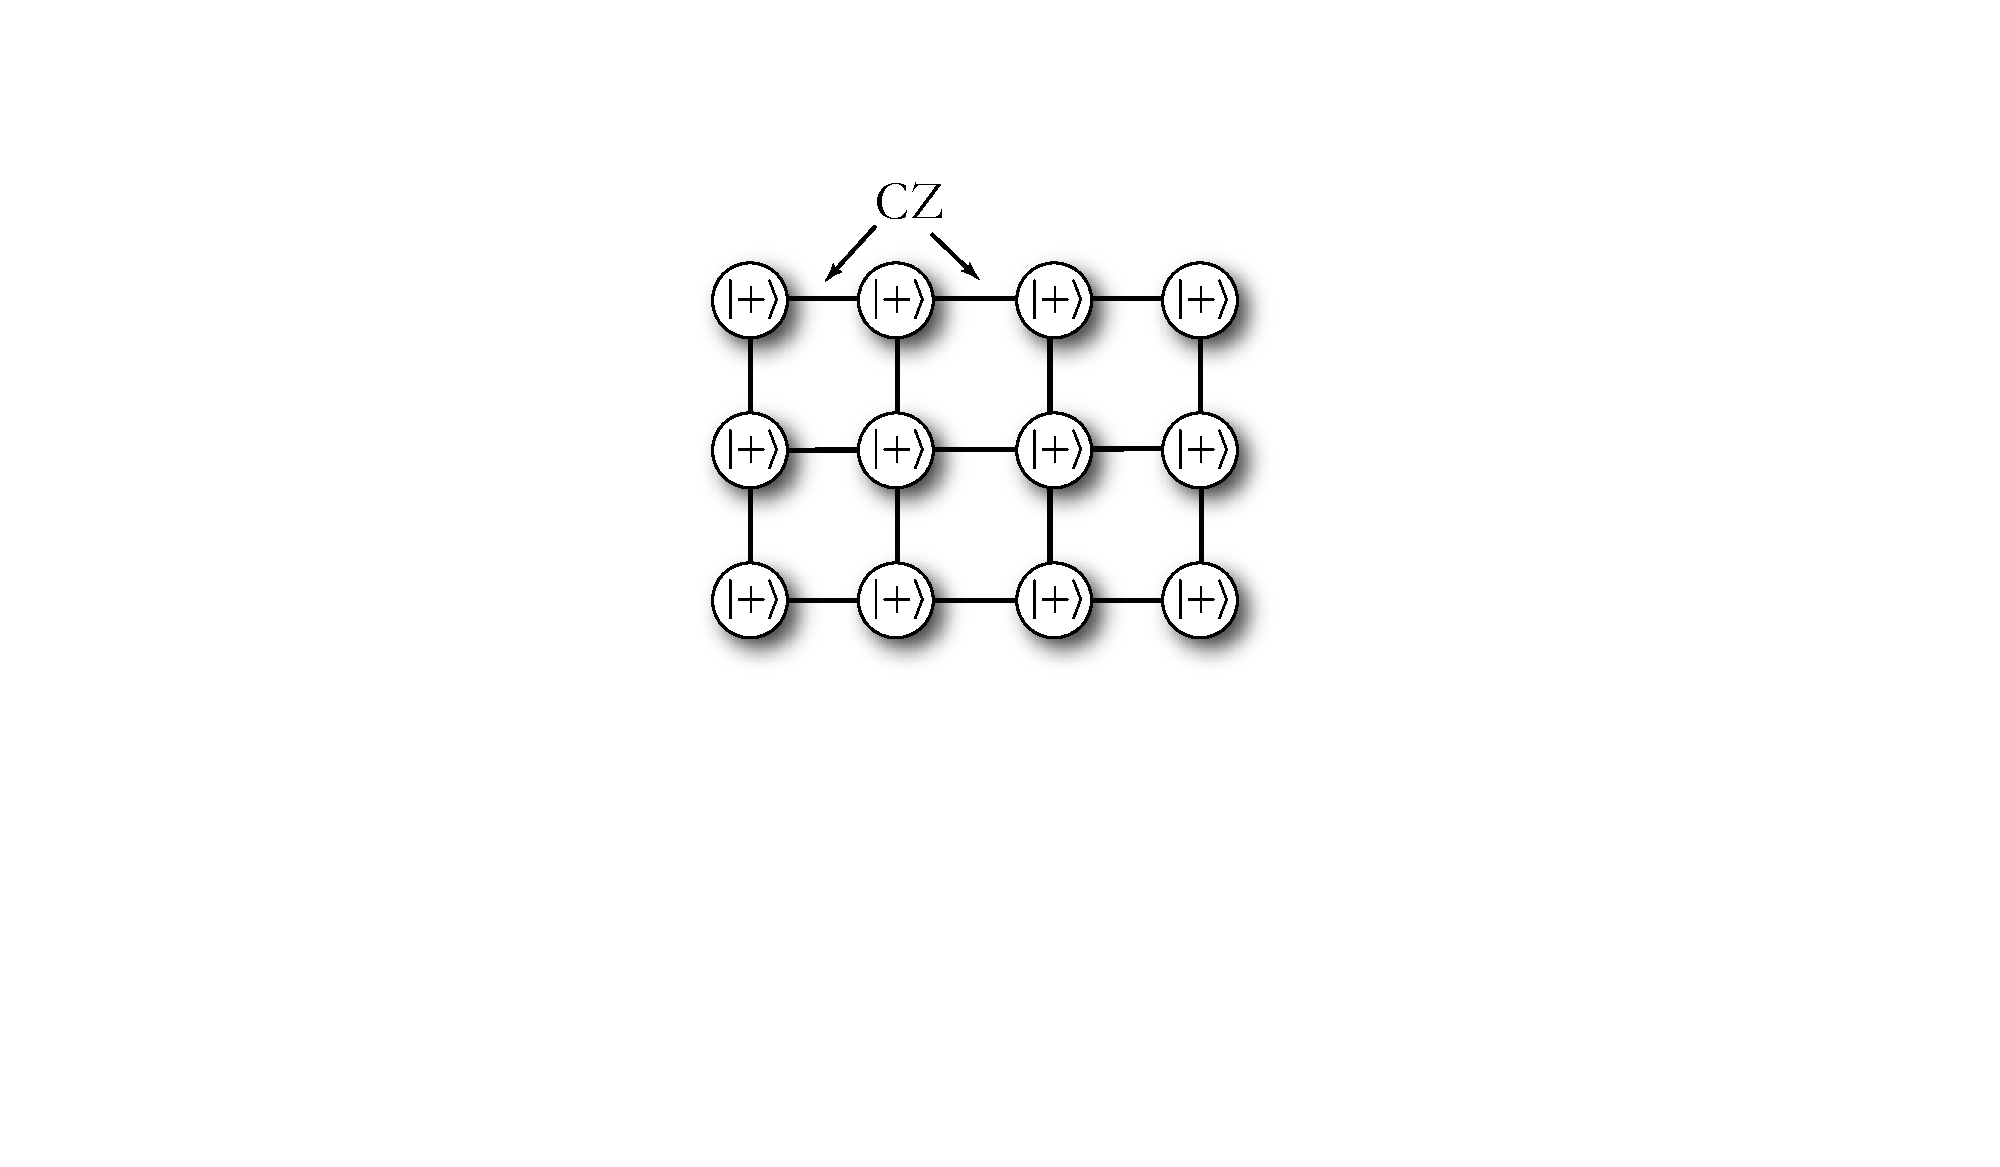
\includegraphics[width=0.3\textwidth]{cluster_state}
	\caption{Example of a \mbox{$4\times 3$} rectangular lattice cluster state. Each vertex in the graph represents a qubit initialised into \mbox{$\ket{+}=\frac{1}{\sqrt{2}}(\ket{0}+\ket{1})$}. Edges represent the application of CZ gates between qubits (CZ gates commute, so the order is unimportant). Of sufficient dimension, states of this topology enable universal measurement-based quantum computation, whereby computation proceeds purely via single-qubit measurements, and all entangling operations have been commuted to the state preparation stage. Because CZ gates commute, the preparation of cluster states is time-independent, and easily implemented in a distributed or parallelised manner. The time-ordering of the single-qubit measurements is dependent on the structure of the graph and the algorithm.} \label{fig:cluster_state}
\end{figure}

Having prepared this state, the computation is implemented purely via a well-orchestrated routine of single-qubit measurements. The order and basis in which they are performed (which depends on previous measurement outcomes in general -- i.e we require fast-feedforward) then stipulates the computation. In the context of distributed computation (Sec.~\ref{sec:dist_QC}), this requires classical communication between nodes.

Mapping a circuit model computation to a cluster state topology can be most na{\" i}vely performed by taking a circuit acting on $n_\mathrm{qubits}$ qubits with depth $n_\mathrm{depth}$, preparing an \mbox{$n_\mathrm{qubits}\times n_\mathrm{depth}$} rectangular lattice cluster, and `etching' the circuit directly into the cluster state substrate. To perform this mapping we choose a universal gate set comprising CZ and single-qubit gates, retaining vertical edges where CZ gates ought to be present, eliminating the remaining vertical edges. Now we have a substrate that looks topologically very much like its equivalent circuit construction, and the computation proceeds chronologically in the same manner. The only conceptual distinction is that in the circuit model gates are directly applied chronologically to the set of qubits, whereas in the cluster state gate teleportation (Sec.~\ref{sec:teleport_gate}) is effectively implemented upon each measurement, with the action of gates accumulating as these teleportations are successively applied. A simple example of this notion is shown in Fig.~\ref{fig:cluster_state_circuit}.

\begin{figure}[!htb]
	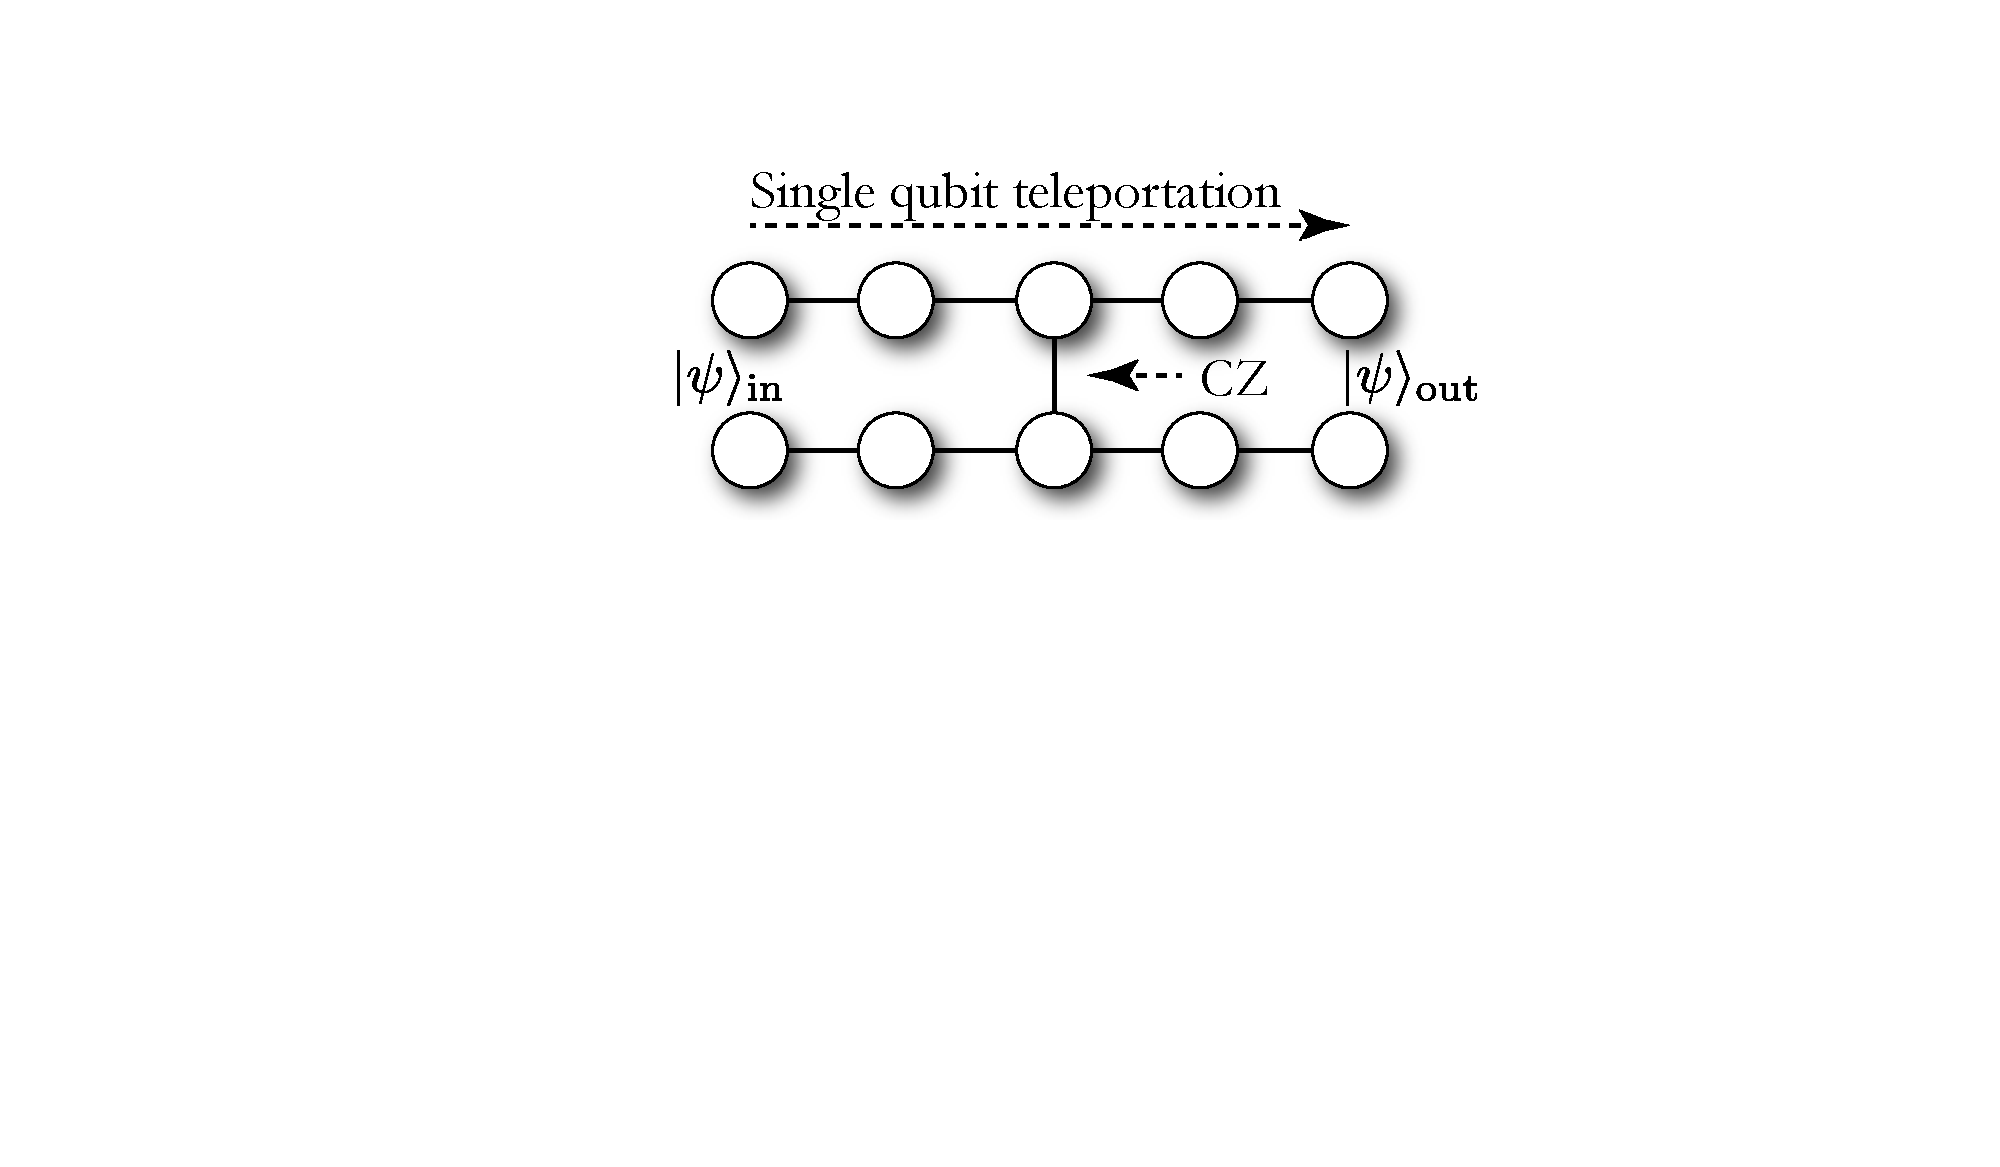
\includegraphics[width=0.375\textwidth]{cluster_state_circuit}
	\caption{Simple example of a cluster state that performs a computation comprising single-qubit operations and a CZ gate between two logical qubits. Let the two horizontal chains represent our two logical qubits. After inputting our input state from the left, we progressively measure out the cluster state qubits chronologically from left-to-right. Upon each single-qubit measurement, the choice of measurement basis teleports the action of a single-qubit gate. These accumulate sequentially. When we reach the point of measuring the two cluster state qubits joined with the vertical edge, the logical qubits accumulate the action of a CZ gate between them, since this is identically what that vertical edge physically corresponds to. Reaching the final two qubits, one from the upper rail and one from the lower, we obtain our two output logical qubits.} \label{fig:cluster_state_circuit}
\end{figure}

The distinctive feature of this model is that all the entangling CZ gates are performed at the very beginning of the protocol, during the state preparation stage. The algorithm itself is purely measurement-based, requiring only single-qubit measurements (no entangling measurements).

An alternate interpretation of the cluster state model is that it is a complicated network of state and gate teleportation protocols (Sec.~\ref{sec:teleport}). Specifically, a CZ gate with a $\ket{+}$ state as a resource, followed by measurement of one of the two qubits acts as a single-qubit teleporter, as shown in Fig.~\ref{fig:single_qubit_teleporter}\footnote{This is an alternative, but equivalent implementation for quantum state teleportation to that presented in Sec.~\ref{sec:teleport}.}. Thus, with a substrate state of CZ gates applied between $\ket{+}$ states, the single-qubit measurements progressively teleport the input state through the graph topology, at each stage accumulating the action of more gates, which are related to the choices of the previous single-qubit measurement bases, and the graph topology.

\begin{figure}[!htb]
	\begin{align}
		\Qcircuit @C=.7em @R=.4em @! {
		\lstick{\ket{\psi}} & \ctrl{1} & \gate{H} & \meter & & \\
		\lstick{\ket{+}} & \ctrl{0} & \qw & \gate{X} \cwx & \gate{H} & \rstick{\ket\psi} \qw \\
		} \nonumber
	\end{align}
	\caption{The single-qubit teleporter, based upon a CZ gate, a single-qubit measurement, and classical feedforward.} \label{fig:single_qubit_teleporter} \index{Single-qubit teleporter}
\end{figure}

The cluster state formalism has proven very useful, enabling the development of models for linear optics quantum computing (Sec.~\ref{sec:KLM_univ}), orders of magnitude more efficient than the originally proposed protocol. It has been found that bonding strategies -- i.e the order in which smaller clusters are fused into larger ones when using non-deterministic gates -- plays a major role in resource overhead, and much work has been performed on efficient preparation strategies for various topologies \cite{bib:Nielsen04, bib:BarrettKok05, bib:BrowneRudolph05, bib:BenjaminEisert05, bib:Gross06, bib:RohdeStratCS07, bib:Kieling06, bib:KielingRudolphEisert06, bib:RohdeBarrett07, bib:Kieling07, bib:Campbell07, bib:Campbell07b}.

These cluster states are highly valuable, given their computational power, and the ability to communicate them from Alice, who is able to prepare them, to Bob, who lacks the technology, would be a boon for Bob.

It would be most practical, economical, and resource efficient to have a single, well-equipped server with the ability to prepare such states, who does so on behalf of everyone else, and communicates the fresh cluster states to them over the quantum internet (for a price, perhaps).

Importantly, the preparation of cluster states is readily parallelised. All the entangling CZ operations commute, the order in which they are applied is irrelevant, and a rectangular lattice cluster is completely uniform. Thus, the graphs representing smaller cluster states may be easily `fused' together to form larger cluster states using, for example, CZ gates. Several other types of entangling gates can also be employed, such as polarising beamsplitters -- so-called \textit{fusion gates} \cite{bib:BrowneRudolph05}. This allows the preparation of cluster states to be performed in a `patchwork quilt'-like manner -- a number of nodes each prepare small lattice clusters, they are all put side-by-side, and stitched together using CZ gates. This type of distributed state preparation is a perfect application for in-parallel distributed quantum processing (Sec.~\ref{sec:dist_QC}).

Consider the scenario whereby Alice requests a large cluster state from Bob, but, while she was unable to prepare the cluster state herself, she has the technological ability to perform the measurement-based computation on the state (i.e simple single-qubit measurements). This would effectively bypass the need for secure quantum computation (Sec.~\ref{sec:homo_blind}) on Bob's hardware altogether, enabling computation with \textit{perfect} secrecy, since no foreign parties would be involved in the computation stage, and no secret data is communicated -- only the \textit{substrate} for the computation is communicated, which could be used for any purpose whatsoever. By commuting all the technologically challenging aspects of a quantum computation to the state preparation stage, we can effectively mitigate the need for blind quantum computing entirely, since the `hard work' has been done in advance by the host, and Alice gets to fulfil the computation on her own, completely bypassing poor old Bob, who was just dying to read Alice's secret love letters before processing them into Hallmark cards.

There are several cluster state identities we will utilise later, summarised in Fig.~\ref{fig:cluster_ident}.

\begin{figure}[!htb]
	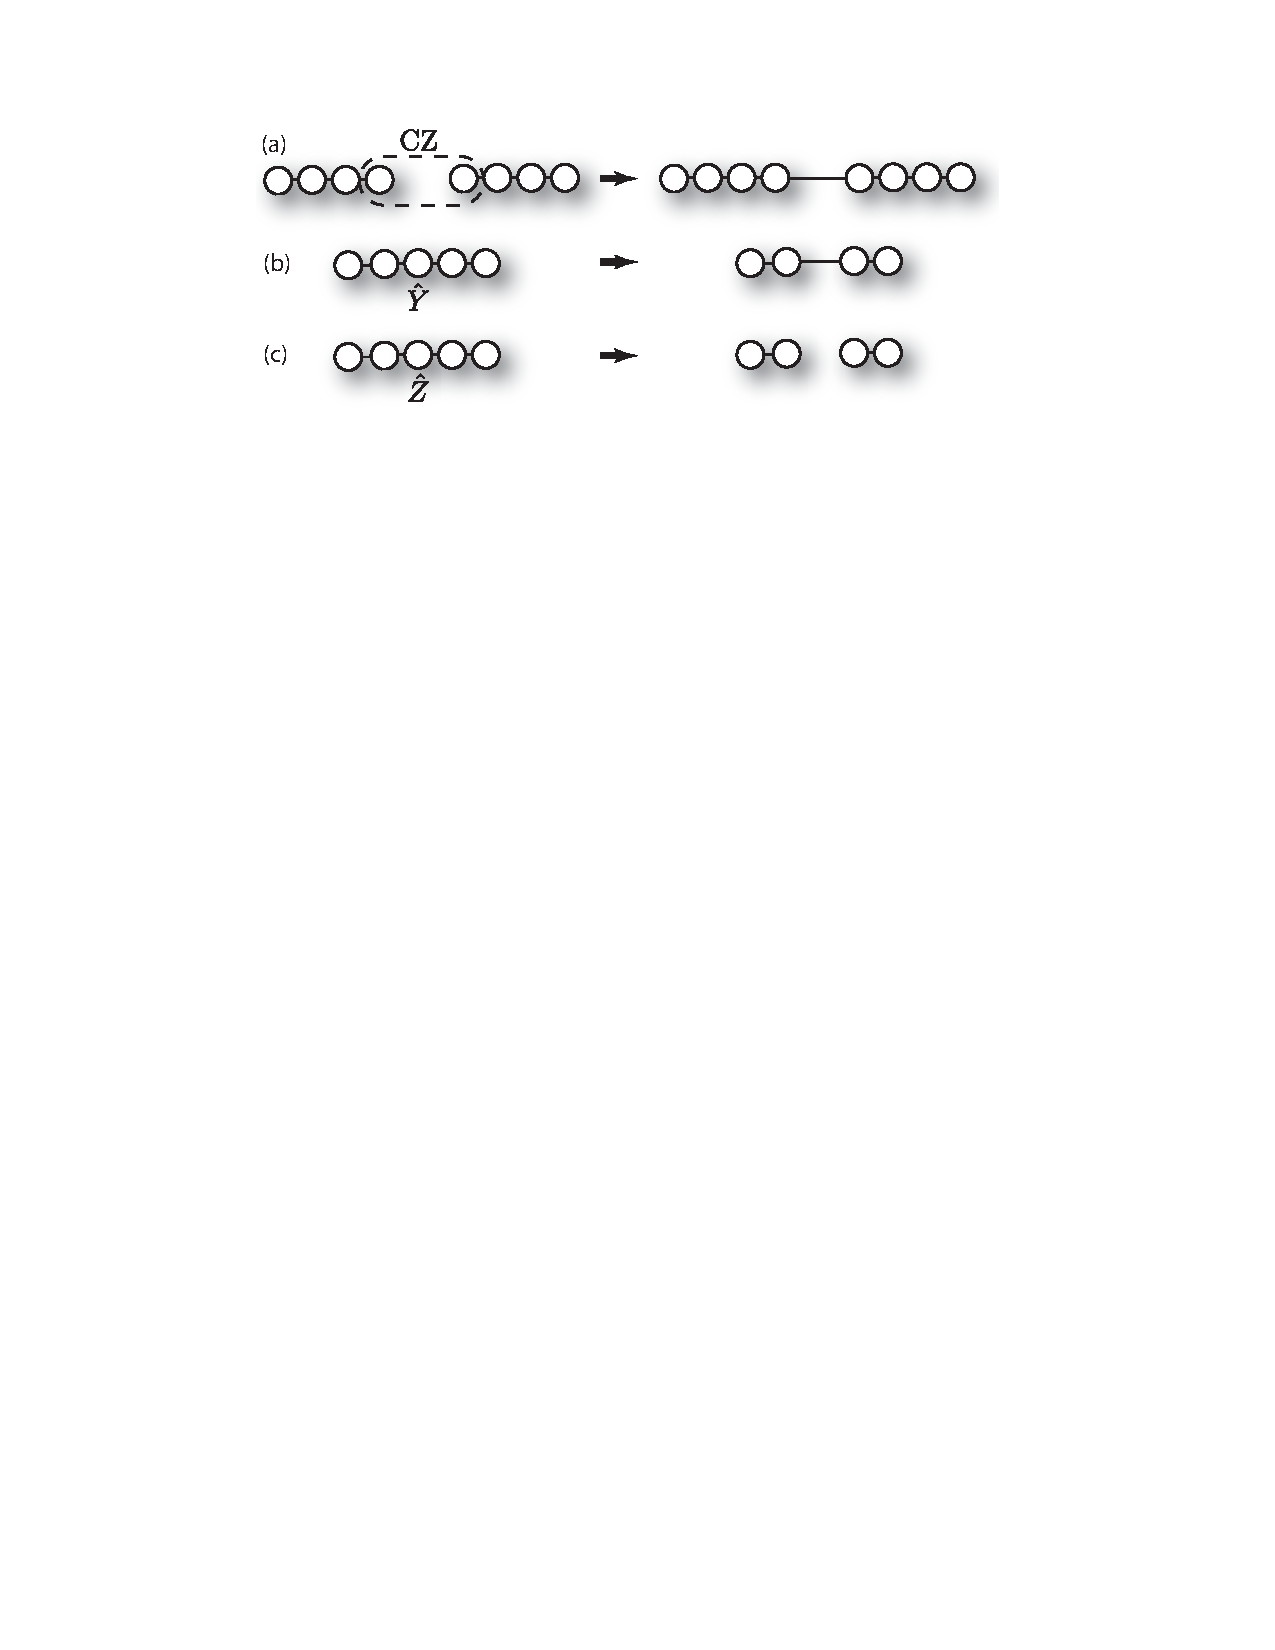
\includegraphics[width=0.47\textwidth]{cluster_identities} \index{Cluster state identities}
	\caption{Several cluster state identities, demonstrated in the case of linear clusters. (a) a CZ gate between two qubits creates an edge between them in the graph. (b) Measurement of a qubit in the Pauli $\hat{Y}$ basis removes that qubit from the graph, whilst creating new edges between the neighbouring qubits. (c) Measurement of a qubit in the Pauli $\hat{Z}$ basis removes that qubit and any neighbouring edges. (d) Measurement of a qubit in the Pauli $\hat{X}$ basis removes that qubit, leaving one of its neighbours as a `dangling node'.} \label{fig:cluster_ident} 
\end{figure}

When using non-deterministic gates (i.e ones that probabilistically fail) to prepare cluster states\index{Non-deterministic cluster staters preparation}, there are approaches to nonetheless preparing ideal cluster states. There have been two main approaches that have become particularly well known. 

The first is to use the ideas of \textit{micro-clusters}\index{Micro-clusters} and cluster state recycling\index{Cluster state recycling} to incrementally build up larger clusters, progressing as a random walk\index{Random walk}, which is biased in the direction of state growth. This approach is discussed in more detail in Secs.~\ref{sec:CS_LO} \& \ref{sec:module}.

The second approach is to borrow techniques from percolation theory\index{Percolation theory} to simply tolerate defects in a cluster state lattice by working around them \cite{Brown}. Specifically, if the defect probability (i.e probability of a missing vertex or edge) is below some \textit{percolation threshold}\index{Percolation threshold}, \mbox{$p_\mathrm{defect}\leq \epsilon_\mathrm{threshold}$}, in the asymptotic limit we are guaranteed that routes exist through the lattice, enabling the required flow of information. This allows defective graphs to be employed for quantum computation.

%
% Adiabatic Quantum Computation & Quantum Annealing
%

\subsection{Adiabatic quantum computation \& quantum annealing} \label{sec:adiabatic_QC} \index{Adiabatic quantum computation} \index{Quantum annealing}

\comment{To do}

%
% Restricted Models for Quantum Computation
%

\subsection{Restricted models for quantum computation} \label{sec:restricted_models} \index{Restricted models for quantum computation}

\comment{To do}

\comment{Talk about Preskill's NISQ or whatever they're called QCs}

%
% Fault-Tolerance
%

\subsection{Fault-tolerance}\index{Fault-tolerance}

\comment{To do. Help from Simon Devitt.}

In Sec.~\ref{sec:QOS_chap} we discussed QoS\index{Quality of service} in the context of quantum networks, where we wish to protect the quantum information being communicated via packets of quantum data. In particular, QEC\index{Quantum error correction} allows us to detect and correct errors introduced into quantum data during transmission across noisy channels.

Much more broadly, in the context of an entire quantum computation we will want to achieve the same goal, except that our techniques will need to extend far beyond defending individual quantum states against errors during transmission, but defending an entire computation and all the information residing within it at every stage throughout its execution.

This is achieved by extending techniques from QEC to achieve \textit{fault-tolerant quantum computing}. The primary difficulty here is that a quantum computation is not a passive operation, but involves the successive application of a potentially enormous number of quantum gates, each of which subject to its own error processes, all of which must be mitigated for the computation to succeed.

Because a quantum computation is not a passive operation but highly active, fault-tolerance protocols are also active and it does not suffice to simply perform an encoding at the beginning and error correction at the end. Instead, error correction procedures must be applied repeatedly throughout execution, at each stage projecting the encoded computation onto an error-free state.

As with conventional QEC, this introduces (potentially large, but efficient) overheads associated with encoding logical qubits into fault-tolerant codes. Similarly, there is the notion of \textit{fault-tolerance thresholds}\index{Fault-tolerance thresholds} -- thresholds on gate error rates that must be achieved if fault-tolerant execution is to be successful. These thresholds are typically depressingly low (well below 1\%) and are the primary reason humanity has not yet achieved scalable quantum computing.